\section{Benchmark Solution}
\label{sec:repOB}
Before introducing new methods designed for \emph{uncertain} graphs, we first consider \emph{somehow} applying existing methods designed for deterministic graphs. 
In this work, we introduce the representative anonymization (Rep-An) algorithm that combines isolated but complementary work from literature for uncertain graph anonymization. 

As shown in Figure~\ref{fig:repOB}, we first extract a \emph{single} \emph{representative} instance from the original uncertain graph. Then, conventional anonymization techniques can be applied on this representative to attain closely approximate anonymized output of the original uncertain graph. There has been extensive work on extracting a single representative instance (deterministic one) of uncertain graphs that capturing graph statistics such as the expected vertex degrees~\cite{Parchas_Gullo_Papadias_Bonchi_2014}. This body of research comes to its aid that anonymization can be carried out on uncertain graphs, regardless of the uncertainty inherent in the data. 

\begin{figure}[t]
  \vspace{-1em}
    \captionsetup{margin=0cm}
    \centering  
        \includegraphics[width=0.95\columnwidth]{AddFigure/repOB.pdf}
        \vspace{-3pt}
      \caption{Overview of Rep-An. Noise is added to the extracted \emph{representative} instance.}
    \label{fig:repOB}
    \vspace{-0.5em}
\end{figure}

\begin{table}[t]
    \centering
        \caption{Characteristics of the datasets and privacy parameters}
        \begin{tabular}{|c|c|c|c||c|}
        \hline 
        Graph    & Nodes    & Edges    &Edge Prob    & Tolerance level\\
        \hline  
        DBLP     &824,774   &5,566,096 & 0.46        & $10^{-4}$\\
        BK       &58,228   & 214,078 &0.29 &$10^{-3}$ \\
        PPI      &12,420   & 397,309  & 0.29         &$10^{-2}$\\
        \hline
        \end{tabular}
        \label{tab:dataset}
\end{table}

\begin{figure}[!htb]
  \subfigure[\small Edge Probability Distribution]{\label{subfig:edgepro}  
    \begin{minipage}[l]{1\columnwidth}
      \centering
       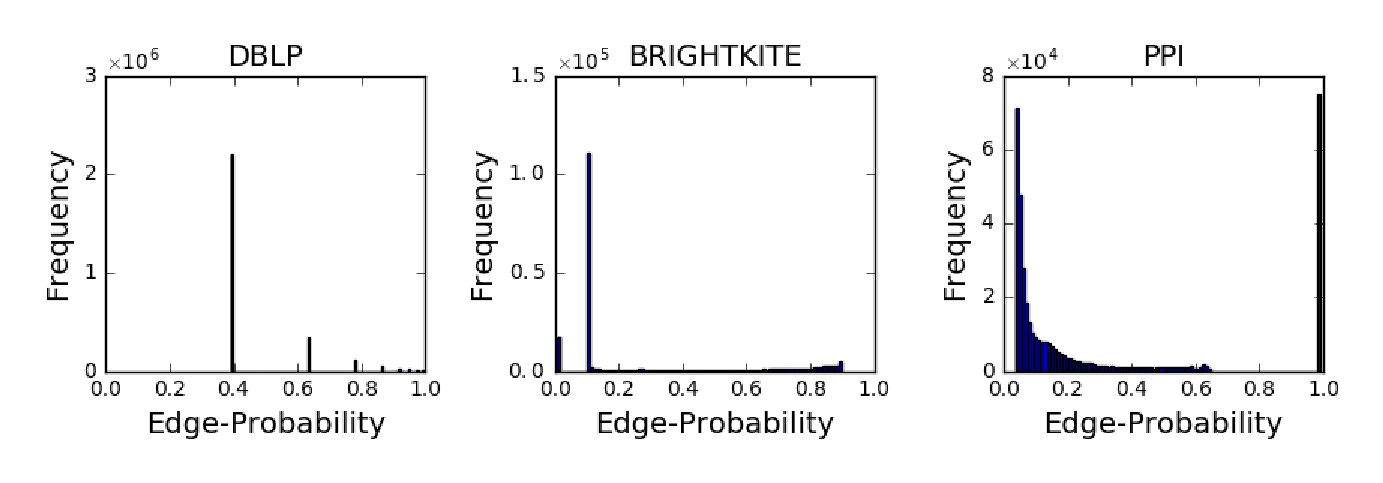
\includegraphics[width=\linewidth]{rep_exp/edge_prob_row.eps}
    \end{minipage}
    \vspace{-15pt}
  }
  \subfigure[\small Expected Degree Distribution]{\label{subfig:degreepro}  
    \begin{minipage}[l]{1\columnwidth}
      \centering
       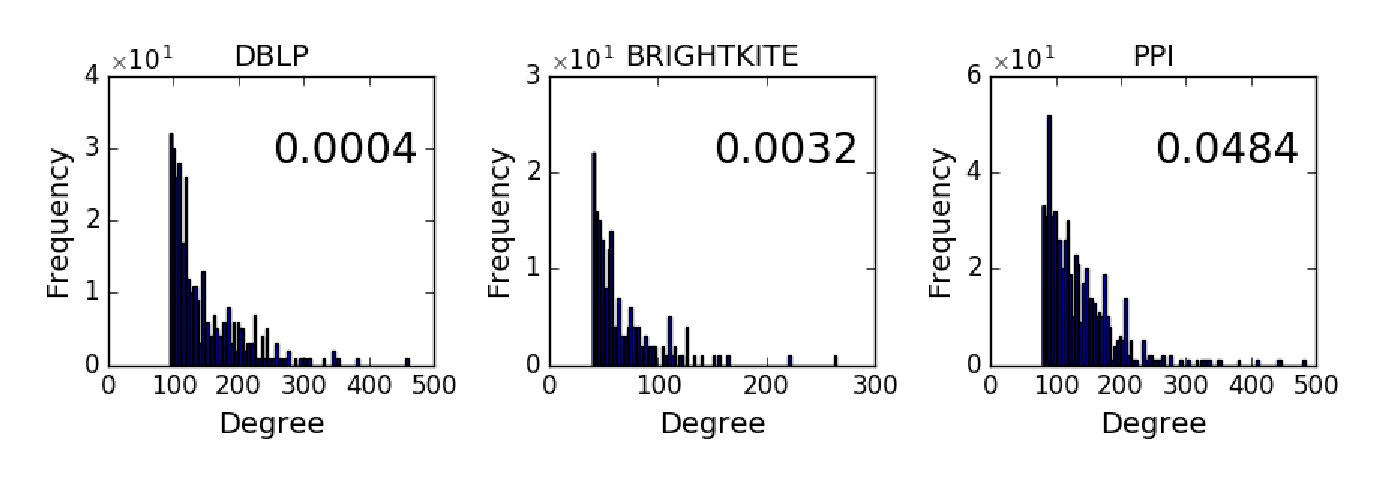
\includegraphics[width=\linewidth]{rep_exp/degree_row.eps}
    \end{minipage}
  }
    \vspace{-5pt}
    \caption{Edge probability\& degree distributions.}
    \label{fig:summary_graph}
   \vspace{-10pt}
\end{figure}


\begin{figure*}[!htb]
    \subfigure[DBLP]{\label{fig:dblp_rep}
      \begin{minipage}[l]{0.62\columnwidth}
        \centering
        \includegraphics[width=1\linewidth]{rep_exp/dblp_rel.pdf}
      \end{minipage}
      }
    \subfigure[\footnotesize{BRIGHTKITE}]{\label{fig:bright_rep}
      \begin{minipage}[l]{0.62\columnwidth}
        \centering
        \includegraphics[width=1\linewidth]{rep_exp/bright_rel.pdf}
      \end{minipage}
      }
      \subfigure[PPI]{\label{fig:ppi_rep}
      \begin{minipage}[l]{0.62\columnwidth}
        \centering
        \includegraphics[width=1\linewidth]{rep_exp/ppi_rel.pdf}
      \end{minipage}
      }

    \vspace{-10pt}
    \caption{The structural distortion introduced for different privacy levels quantifies as the average reliability discrepancy between the original ones and perturbed ones.}
    \label{fig:rep_exp}
    \vspace{-15pt}
\end{figure*}

However, this approach has several limitations. First, the input edge uncertainties (probabilities) are no longer integrated into the anonymization process since they are detached from the graph in the first step. Second, since the two phases are isolated from each other, different phases might be optimized for different metrics. As the result, this benchmark solution Rep-An introduces a high level of noise and consequently deteriorates the overall utility.

\subsection{Validation on Real Uncertain Graphs}
In this section, we empirically evaluate the impact of noise injected to extracted \emph{representative} instances on real uncertain graphs. 

\textbf{Uncertain Graph Collections.}~~We use three uncertain graphs that capture different real-world scenarios and have been used in prior uncertain graph mining studies. Table~\ref{tab:dataset} lists uncertain graphs and their tolerance parameters used in our evaluation.

\textsc{DBLP}~\cite{dblps} is a co-authorship network where the probability of an edge between two authors represents the likelihood two authors will collaborate in the future. The probability is obtained by a predictive model based on historical co-authorship data~\cite{Jin_Distance_2011}. 

\textsc{BrightKite}~\cite{snapnets} is a location-based social network where the probability of an edge between two users corresponds to the chance that two users visit each other. The probability can be obtained by a prediction model based on historical user location data~\cite{Cho_Friendship_2011}. Generally, location data is considered to be sensitive because of personal security issues. 

\textsc{PPI} is a dataset of protein-protein interactions, provided by Disease Module Identification DREAM Challenge, where the probability of any edge corresponds to the confidence that the interaction actually exists.
The probability is obtained through biological experiments.

% Add one sentence 
Figure~\ref{subfig:edgepro} shows the edge-probability distribution in these three datasets. 
Note that the DBLP dataset only has a few probability values distributed in $[0,1]$, while Brightkite dataset's probability values are generally very small. The PPI dataset has a more uniform probability distribution. 
We also present their degree distributions of ``unique'' nodes (with high degree and obfuscation level is smaller than $300$). Observe that, all the three graphs have a heavy-tailed degree distribution (i.e, an amount of ``unique" nodes). The larger amount of ``unique'' nodes requires a larger amount of noise.


% pass 
\textbf{Computation.}~~We first extract the single representative instances for each uncertain graph, introduce noise using the state-of-art graph anonymization approach~\cite{Boldi_Injecting_2012}, and then compute the Average Reliability Discrepancy between the perturbed graph and the original uncertain graph as a measure of the level of graph structural error introduced. We approximate its expectation value by the average value obtained over the sampled possible worlds. Here, we use 1,000 samples since it has been shown that $1000$ usually suffices to achieve accuracy converge~\cite{Potamias_K_2010}.

\textbf{Results.}~~Figure~\ref{fig:rep_exp} shows that the Rep-An algorithm produces a large error for large values of $k$ (i.e. strong privacy guarantees). As we mentioned, the low level of utility is due to the large noise Rep-An injects into the representative instance, resulting in a perturbed graph (uncertain one) which is significantly different from the original \emph{uncertain} graph. 

To better understand the limitation of Rep-An, we report the potential lower-bound on the error that could be achieved via Chameleon methods in Figure~\ref{fig:rep_exp}. Figure~\ref{fig:rep_exp} shows that the utility loss of the Rep-An strategy can largely be attributed to the overlook of edge uncertainty. 
The large deviation is largely due to the representative extraction step. In the extreme case where $k=100$ (i.e. weak privacy guarantee requires little noise), the sole representative extraction step produces high reliability errors (i.e, structural distortion). 

The \textsc{DBLP} graph shows a more evident gap. For small $k$ values, i.e., $k=100$ and $k=150$, the largest error is within 30\% from the original graph values. The \textsc{DBLP} graph shows a more evident gap because the representative extraction processing alters a large amount of edge probability, consequently, introduces huge structural change. 
% add one sentence about the
% add more sentences to highlight their difference. 




